\documentclass[letterpaper, 12pt]{report}
\usepackage[utf8]{inputenc}
\usepackage{amsmath,amssymb,amsthm}
\usepackage[spanish]{babel}
\usepackage{graphicx}
\usepackage{caption}
\usepackage{subcaption}
\usepackage{xcolor}
\usepackage{titlesec}
\usepackage{lmodern}
\usepackage{fancyhdr}
\usepackage{geometry}


\usepackage{algorithm}
\usepackage{algpseudocode}
\usepackage{multirow}
\usepackage{booktabs}

\setlength{\headheight}{24.01996pt}
\addtolength{\topmargin}{-12.01996pt}

% Definir colores personalizados
\definecolor{primary}{RGB}{25,55,95}
\definecolor{secondary}{RGB}{200,35,45}

% Configurar márgenes
\geometry{
    left=3cm,
    right=2.5cm,
    top=3cm,
    bottom=2.5cm
}

\newtheorem*{theorem*}{Teorema}

% Configurar estilo de títulos
\titleformat{\chapter}[display]
{\normalfont\Huge\bfseries\color{primary}}
{\chaptertitlename\ \thechapter}{20pt}{\Huge}

\titleformat{\section}
{\normalfont\Large\bfseries\color{primary}}
{\thesection}{1em}{}

% Configurar encabezado y pie de página
\pagestyle{fancy}
\fancyhf{}
\fancyhead[L]{\small\textcolor{primary}{\nouppercase{\leftmark}}}
\fancyfoot[C]{\textcolor{primary}{\thepage}}
\renewcommand{\headrulewidth}{0.4pt}
\renewcommand{\headrule}{\hbox to\headwidth{\color{primary}\leaders\hrule height \headrulewidth\hfill}}

% Portada personalizada
\newcommand*{\customtitlepage}{
    \begin{titlepage}
        \begin{center}
            \vspace*{1cm}
            
            
            {\LARGE \textbf{UNIVERSIDAD DE LA HABANA}}\\
            \vspace{0.5cm}
            {\Large Facultad de Matem\'atica y Computaci\'on}\\
            

            
\includegraphics[scale=0.5]{images/logo.png}
            
            \vspace{1cm}
            
            
            \rule{\textwidth}{1.5pt}\\
            \vspace{0.5cm}
            {\LARGE \textcolor{primary}{\textbf{PROYECTO FINAL}}}\\
            {\LARGE \textcolor{primary}{\textbf{DISE\~NO Y AN\'ALISIS DE ALGORITMOS}}}
            \vspace{0.5cm}
            \rule{\textwidth}{1.5pt}
            
            \vspace{2cm}
            
            {\Large \textbf{Diseño Computacional de Prote\'inas}}\\
            \vspace{1cm}
            
            {\Large \textbf{Autor:} Lidier Robaina Caraballo \\
            \vspace{0.5cm}
            {\Large \textbf{Grupo:} C-411 }\\
            \vspace{1.5cm}
            
            {\Large \today}
            }
        \end{center}
    \end{titlepage}
}

\begin{document}

\customtitlepage

% Índice
\tableofcontents
\thispagestyle{empty}
\cleardoublepage

% Contenido principal
\setcounter{page}{1}

\chapter{Introducción}

La bioinform\'atica emerge como un campo revolucionario en la intersección entre la biología, la química y la ciencia de la computación, ofreciendo herramientas innovadoras para abordar desafíos científicos y tecnológicos de alto impacto. Las proteínas, como máquinas moleculares esenciales para la vida, desempeñan roles críticos en procesos biológicos, aplicaciones médicas (como el desarrollo de fármacos y terapias) y soluciones industriales (como biocatalizadores y materiales biodegradables). Sin embargo, el diseño tradicional de proteínas, basado en métodos experimentales de ensayo y error, resulta costoso, lento y limitado en complejidad. Aquí es donde los algoritmos computacionales se convierten en un aliado indispensable: permiten modelar, predecir y optimizar estructuras proteicas con precisión, acelerando el descubrimiento de soluciones biológicas personalizadas.  \\

La \textbf{motivación} de este proyecto radica en dos pilares fundamentales. Primero, la necesidad de explorar estrategias algorítmicas eficientes para resolver problemas NP-duros asociados al diseño de proteínas, como el plegamiento tridimensional y la estabilidad termodinámica. Segundo, la oportunidad de contribuir al avance de áreas como la medicina personalizada, la bioingeniería y la sostenibilidad ambiental, donde proteínas diseñadas a la medida podrían transformar paradigmas actuales. \\

Los \textbf{objetivos} del proyecto se centran en:
\begin{itemize}
    \item[1.] Modelar el problema de diseño de proteínas desde una perspectiva algorítmica, identificando sus componentes críticos (espacio de búsqueda, funciones de energía, restricciones biológicas).  
    \item[2.] Analizar la complejidad del problema.
    \item[3.] Implementar un algoritmo que resuelva el problema de forma exacta, evaluando su eficiencia (tiempo y espacio).   
\end{itemize}



\chapter{Definici\'on del Problema DCP}

\section{Marco Te\'orico}

Las proteínas son macromol\'eculas esenciales para la vida dado que est\'an involucradas en casi todas las funciones estructurales,
catal\'iticas, sensoriales y regulatorias de los organismos. Est\'an formadas por una secuencia de compuestos org\'anicos llamadas aminoácidos,
y su función está determinada fundamentalmente por la estructura tridimensional que adopta la cadena de aminoácidos. \\  

El objetivo del diseño de proteínas es encontrar, dentro de una colección de proteínas, la que m\'as probabilidades tiene de ajustarse a una función.
Puesto que existen veinte aminoácidos posibles para cada posición en una secuencia proteica, y cada uno de ellos admite diversas variantes estructurales, 
la cantidad de combinaciones factibles a evaluar supera las posibilidades de cualquier método experimental, incluso en el caso de secuencias muy cortas.


\subsection{Esqueleto}

Como ilustra la figura \ref{fig1}, los aminoácidos est\'an formado por un n\'ucleo com\'un (\'atomos de H, C, N y O) y una
cadena lateral (R) que es espec\'ifica para cada uno de los 20. En una proteína, los núcleos de los amino\'acidos están
enlazados en una secuencia que forma el \textit{esqueleto} de la proteína. \\



El esqueleto es relativamente r\'igido y define la estructura tridimensional de la proteína (figura \ref{fig2}), por tanto se asume
que la proteína resultante del diseño conservar\'a el plegamiento global de la estructura base elegida. Es decir,
se considera que el esqueleto de la proteína está fijo y es entrada del problema del diseño de proteínas. \\

\newpage

\begin{figure}[h!]
    \begin{center}
        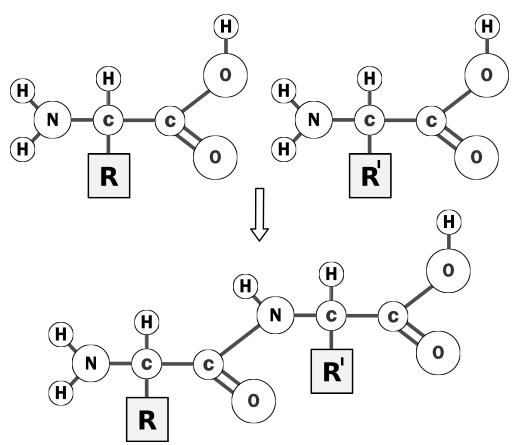
\includegraphics[scale=0.5]{images/dipeptido.png}
    \end{center}    
    \caption{Representaci\'on de c\'omo dos aminoácidos, con cadenas laterales espec\'ificas $R$ y $R'$, enlazan sus n\'ucleos para formar una cadena}
    \label{fig1}
\end{figure} 

\begin{figure}[h!]
    
    \begin{subfigure}[b]{0.49\textwidth}
        \begin{center}
            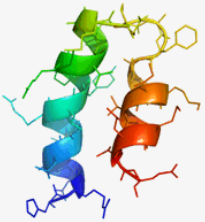
\includegraphics[scale=0.8]{images/protein.png} 
            \caption{Modelo con cadenas laterales}  
        \end{center}              
    \end{subfigure}    
    \begin{subfigure}[b]{0.49\textwidth}
        \begin{center}
            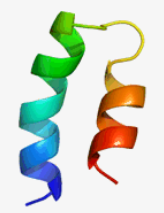
\includegraphics[scale=0.8]{images/backbone.png}  
            \caption{Esqueleto}  
        \end{center}             
    \end{subfigure}
    \caption{Modelo 3D de una proteína}
    \label{fig2}
\end{figure}









\subsection{Rot\'ameros}

Debido a la rotaci\'on alrededor de los enlaces simples, las cadenas laterales de los aminoácidos pueden adoptar distintas
conformaciones tridimensionales, que reciben el nombre de \textit{rotámeros}. Hay una cantidad 
infinita de rotámeros posibles, puesto que las moléculas pueden girar alrededor del eje de forma continua.
No obstante, suele ser suficiente considerar un conjunto discreto y representativo de rotámeros (figura \ref{fig3}),
el cual se puede determinar a través de un análisis estadístico de las conformaciones reales presentes en las 
bases de datos de estructuras de proteínas. \\

En el problema del diseño de proteínas, los rotámeros constituyen el espacio de b\'usqueda primario cuando el esqueleto está fijo.


\begin{figure}
    \begin{center}
        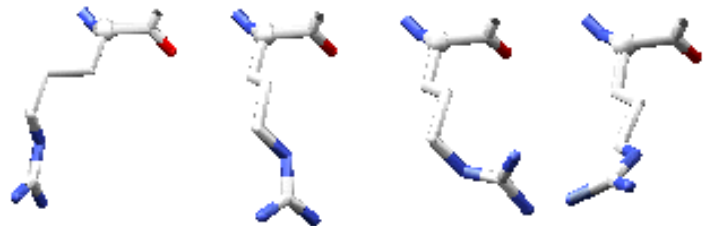
\includegraphics[scale=0.5]{images/rotameros.png}
    \end{center}    
    \caption{Rotámeros del aminoácido arginina: algunas posibles geometr\'ias de la cadena lateral}
    \label{fig3}
\end{figure} 

\subsection{Funciones de energ\'ia}

La estabilidad y la eficiencia funcional de una proteína están correlacionadas con su energía, por lo tanto, el objetivo
es encontrar la conformación que posea la energía total mínima. \\

La energía total de la proteína está dada por la energía del esqueleto, la energía de interacción entre los rotámeros y el esqueleto,
y la energía de interacción entre los diferentes rotámeros. Cuando el esqueleto está fijo, la minimización de la energía 
depende únicamente de la energía de interacción entre los rotámeros y entre estos y el esqueleto.
Sean $i_r$ el rotámero en la posición $i$, $E(i_r)$ la energía de interacción entre el rotámero $i$ y el esqueleto, 
y $E(i_r , j_{r'})$ la energía de interacción entre los rotámeros $r$ en la posición $i$ y $r'$ en la posición $j$, la fórmula a minimizar se convierte en

\[E = \sum_i E(i_r) + \sum_i \sum_{j<i} E(i_r , j_{r'})  \]

%Los valores de energía normalmente se miden en kcal/mol y deben ser precomputados y almacenados en memoria.


\section{Modelaci\'on como problema de teor\'ia de grafos}


 
Una proteína con $k$ aminoácidos puede ser representada por un grafo $k$-partito $G = (V,E)$, de forma tal que:
\begin{itemize}
    \item hay una partición $V_i$ por cada aminoácido $i$
    \item hay un vértice $v \in V_i$ por cada rotámero candidato del aminoácido $i$
    \item la arista $\langle u,v \rangle$ denota la interacción entre los rotámeros $u$ y $v$
    \item el vértice $v$ tiene un costo $c_v$ que es igual a la energía de interacción entre el rotámero $v$ y el esqueleto
    \item la arista $\langle u,v \rangle$ tiene un costo $c_{ \langle u,v \rangle }$ que es igual a la energía de interacción entre el rotámero $u$ y el rotámero $v$ \\
\end{itemize}

Cada rotámero puede potencialmente interactuar con cualquier rotámero de cualquier otra posición distinta a la suya, por
por tanto  $G$ es un grafo $k$-partito completo. Luego, seleccionar un rotámero para cada aminoácido es equivalente a seleccionar
un clique de tamaño máximo (necesariamente tamaño $k$) (figura \ref{fig4}). \\

\begin{figure}[h!]
    \begin{center}
        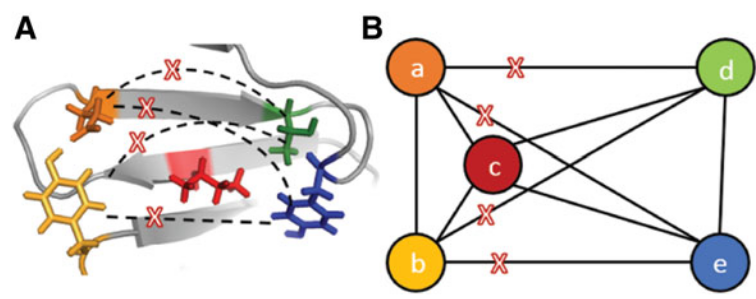
\includegraphics[scale=0.7]{images/solution.png}
    \end{center}    
    \caption{\textbf{(A)} Ejemplo de diseño de una proteína, cada color corresponde a una partición del grafo \textbf{(B)} Ejemplo de clique solución del problema A}
    \label{fig4}
\end{figure} 

El problema del \textbf{Dise\~no Computacional de Proteínas (DCP)} se define como:

\begin{quote}
    Dado un grafo $k$-partito completo $G = (V,E)$, $V = V_1 \cup V_2 \cup ... \cup V_k$, ponderado en vértices y aristas, hallar el 
    clique $C$ de tamaño $k$ tal que el grafo inducido por $C$ es de costo m\'inimo. \\
    
    Lo anterior es equivalente a seleccionar un $v_i \in V_i \ \forall \ 1 \leq i \leq k$, tal que  
    \[E_{total} = \sum_i c_{v_i} + \sum_i \sum_{j<i} c_{ \langle v_i,v_j \rangle }  \]
    sea m\'inima.
\end{quote}


\chapter{An\'alisis de complejidad}


\section{DCP $\in$ NP-Hard}



\subsection{Definiciones}


\begin{itemize}
    \item \textbf{Clique(G,k)}: Dado un grafo $G$ y un entero $k$, determinar si en $G$ existe un clique de tamaño $k$.
    \item \textbf{DCP\_E(G,E)}: Dado un grafo $n$-partito completo $G$ y una constante $E$, determinar si $G$ tiene un clique
    de tamaño $n$ y costo $E_{total} \leq E$.
\end{itemize}

\subsection{Reducción Clique $\propto$ DCP\_E}

Sea $(G=(V,E),k)$ una instancia de Clique, $n=|V|$, se construye un grafo $n$-partito completo $G'$  como sigue:

\begin{itemize}
    \item[1.] Particiones de $ G' $
    \begin{itemize}
        \item Cada vértice $ v_i \in V $ corresponde a una partición $ V_i $ en $ G' $.  
        \item Cada partición $ P_i $ tiene dos vértices:  
        \begin{itemize}
            \item $ a_i $ (representa incluir $ v_i $ en el clique), con peso 0. 
            \item $ b_i $ (representa excluir $ v_i $), con peso 1.  
        \end{itemize}
    \end{itemize}
    \item[2.] Aristas en $ G' $
    \begin{itemize}
        \item Para cada par de particiones $ V_i, V_j $ ($ i \neq j $): 
        \begin{itemize}
            \item Si $ \langle v_i, v_j \rangle \in E $, la arista $ \langle a_i, a_j \rangle $ tiene peso 0.  
            \item Si $ \langle v_i, v_j \rangle \notin E $, la arista $ \langle a_i, a_j \rangle $ tiene peso 1.  
        \end{itemize}
        \item Todas las aristas que involucran algún $ b_i $ tienen peso $ 0 $.  
    \end{itemize}    
\end{itemize}

% 1. **Particiones de $$ G' $$**:  
%    - Cada vértice $$ v_i \in V $$ corresponde a una partición $$ P_i $$ en $$ G' $$.  
%    - Cada partición $$ P_i $$ tiene dos vértices:  
%      - $$ a_i $$ (representa "incluir $$ v_i $$ en la clique"), con peso $$ 0 $$.  
%      - $$ b_i $$ (representa "excluir $$ v_i $$"), con peso $$ M $$ ($$ M \gg 0 $$).  

% 2. **Pesos de aristas en $$ G' $$**:  
%    - Para cada par de particiones $$ P_i, P_j $$ ($$ i \neq j $$):  
%      - Si $$ (v_i, v_j) \in E $$ en $$ G $$, la arista $$ (a_i, a_j) $$ tiene peso $$ 0 $$.  
%      - Si $$ (v_i, v_j) \notin E $$, la arista $$ (a_i, a_j) $$ tiene peso $$ M $$.  
%    - Todas las aristas que involucran algún $$ b_i $$ tienen peso $$ 0 $$.  

% ---

\subsection{Equivalencia de soluciones}

\begin{theorem*}
    $G$ tiene un clique de tamaño $k$ si y solo si $G'$ tiene un clique de tamaño $n$ y costo $E_{total} \leq 0$ .
\end{theorem*}

\noindent
\textbf{Demostración} \\


($\Rightarrow$) \\


Seleccionando los vértices $ a_i $ correspondientes a los $ k $ nodos del clique en $ G $, el conjunto formado por esos v\'ertices es un clique de tamaño $n$ y cumple que:  

\begin{itemize}
    \item Los vértices $ a_i $ tienen peso 0.  
    \item Las aristas entre ellos tienen peso 0 (porque forman un clique en $ G $).  
\end{itemize}

Por tanto, tiene costo $E_{total} = 0 \leq 0$. \\

($\Leftarrow$) \\ 
Seleccionando el clique en cuesti\'on:
\begin{itemize}
    \item Todos los vértices del clique deben ser $ a_i $ (ya que cualquier $ b_i $ añadiría peso).
    \item Las aristas entre estos $ a_i $ deben tener peso 0, lo que implica que $ \langle v_i, v_j \rangle \in E $ para todo par.      
\end{itemize}

Esto corresponde a un clique de tamaño $ k $ en $ G $.  $\square$

Dado que Clique es un conocido problema NP-Completo, con la reducción anterior se ha demostrado que DCP\_E es un problema
NP-Hard. También es f\'acil comprobar que DCP\_E es NP, por tanto, es NP-Completo. Luego, como DCP es un problema
de optimización correspondiente a un problema de decisi\'on NP-Completo, $DCP \in NP-Hard$




% ---

% ### **Argumentos de complejidad**
% 1. **Construcción polinomial**:  
%    - $$ G' $$ tiene $$ 2|V| $$ vértices y $$ O(|V|^2) $$ aristas.  
%    - Los pesos se asignan en tiempo constante por arista.  

% 2. **Preservación de soluciones**:  
%    - Un algoritmo para el problema de diseño de proteínas resolvería Clique en tiempo polinomial, lo que es imposible a menos que $$ P = NP $$.  

% ---

% ### **Ejemplo ilustrativo**
% Considere $$ G $$ con vértices $$ \{1, 2, 3\} $$ y aristas $$ \{(1,2), (2,3)\} $$. Queremos ver si existe una clique de tamaño $$ k=2 $$.  
% - En $$ G' $$:  
%   - Particiones: $$ P_1 = \{a_1, b_1\}, P_2 = \{a_2, b_2\}, P_3 = \{a_3, b_3\} $$.  
%   - Aristas con peso $$ 0 $$: $$ (a_1, a_2) $$, $$ (a_2, a_3) $$.  
%   - Aristas con peso $$ M $$: $$ (a_1, a_3) $$.  
% - **Solución**: Seleccionar $$ a_1, a_2 $$ (clique en $$ G $$) → peso total = 0.  

% ---

% \section{Irreducibilidad de DCP}


% \chapter{Conclusiones}

% Al integrar fundamentos algorítmicos con desafíos biológicos, este proyecto no solo busca profundizar en el entendimiento teórico de problemas de optimización complejos, sino también demostrar cómo el diseño computacional puede catalizar innovaciones prácticas en bioingeniería.


\section{DCP no es aproximable}

Supondremos la existencia de un algoritmo de aproximación con factor constante $\alpha \geq 1$ y mostraremos que esto permitiría resolver 3-SAT en tiempo polinomial, contradiciendo la NP-dureza del problema.


\subsection{Reducción 3-SAT $\propto$ DCP}
Para cualquier $\alpha \geq 1$, construimos un grafo $m$-partito completo $G$ desde una fórmula 3-CNF $\phi$ con $m$ cláusulas:

\begin{itemize}
    \item \textbf{Particiones}: $m$ particiones (uno por cláusula)
    \item \textbf{Nodos}: 3 por partición (literales de la cláusula)
    \item \textbf{Pesos en nodos}: $1$ para todos los nodos
    \item \textbf{Pesos en aristas}:
    \[
    w(u,v) = 
    \begin{cases}
        0, & \text{si } u \text{ y } v \text{ son consistentes} \\
        W, & \text{con } W = \lceil (\alpha - 1)m \rceil + 1 \quad (\text{para literales inconsistentes})
    \end{cases}
    \]
\end{itemize}

\subsection{Análisis de Costos}
\begin{itemize}
    \item Caso 1: $\phi$ es satisfacible
    \begin{itemize}
        \item \textbf{Costo nodos}: $m \times 1 = m$
        \item \textbf{Costo aristas}: $0$ (sin inconsistencias)
        \item \textbf{OPT} = $m$
    \end{itemize}
    \item Caso 2: $\phi$ no es satisfacible
    \begin{itemize}
        \item \textbf{Costo nodos}: $m \times 1 = m$
        \item \textbf{Costo aristas}: $\geq W$ (al menos una inconsistencia)
        \item \textbf{OPT} $\geq m + W = m + \lceil (\alpha - 1)m \rceil + 1 \geq \alpha m + 1$
    \end{itemize}
\end{itemize}


\subsection{Ratio de Aproximación}
Para cualquier algoritmo $\mathcal{A}$ con factor $\alpha$:
\[
\frac{\text{Costo}(\mathcal{A}(G))}{\text{OPT}} \leq \alpha
\]
Esto implica:
\[
\begin{cases}
\mathcal{A}(G) \leq \alpha m & \text{si } \phi \text{ es satisfacible} \\
\mathcal{A}(G) \geq \alpha m + 1 & \text{si } \phi \text{ no es satisfacible}
\end{cases}
\]

\subsection{Contradicción}
Un algoritmo $\alpha$-aproximado distinguiría entre los dos casos en tiempo polinomial:
\begin{enumerate}
    \item Si $\mathcal{A}(G) \leq \alpha m \Rightarrow \phi$ es satisfacible
    \item Si $\mathcal{A}(G) \geq \alpha m + 1 \Rightarrow \phi$ no es satisfacible
\end{enumerate}

Esto resolvería 3-SAT en tiempo polinomial, por tanto DCP no puede ser aproximado dentro de ningún factor constante salvo que P = NP.





\chapter{Solución}



\section{Branch and Bound (B\&B)}

El algoritmo B\&B construye progresivamente el clique seleccionando un residuo por partición. En cada paso:

\begin{itemize}
\item \textbf{Ramificación}: Genera subproblemas al elegir diferentes nodos de la partición actual
\item \textbf{Acotamiento}: Calcula una cota inferior (LB) del costo mínimo posible para completar el clique
\item \textbf{Poda}: Si LB $\geq$ mejor solución actual, abandona esa rama
\end{itemize}


\subsection{Pseudocódigo}
\begin{algorithm}[H]
\caption{Branch and Bound para DCP}
\begin{algorithmic}[1]
\State \textbf{Entrada:} Grafo $k$-partito completo con costos en nodos y aristas
\State \textbf{Salida:} Clique de costo mínimo
\State Inicializar \texttt{mejor\_costo} $\leftarrow \infty$
\Procedure{BranchAndBound}{$S$, $costo$, $P$}
    \If{$P = \emptyset$}
        \If{$costo < \texttt{mejor\_costo}$}
            \State Actualizar solución óptima
        \EndIf
        \Return
    \EndIf
    \State Seleccionar partición $p \in P$
    \For{cada nodo $v \in p$}
        \State $nuevo\_costo \leftarrow costo + C(v) + \sum_{u \in S}C(u,v)$
        \State $lb \leftarrow$ \textsc{CotaInferior}($S \cup \{v\}$, $P \setminus \{p\}$)
        \If{$nuevo\_costo + lb < \texttt{mejor\_costo}$}
            \State Llamar recursivamente \textsc{BranchAndBound}
        \EndIf
    \EndFor
\EndProcedure
\end{algorithmic}
\end{algorithm}

% El algoritmo B\&B construye progresivamente el clique seleccionando un residuo por partición. En cada paso:

% \begin{itemize}
% \item \textbf{Ramificación}: Genera subproblemas al elegir diferentes nodos de la partición actual
% \item \textbf{Acotamiento}: Calcula una cota inferior (LB) del costo mínimo posible para completar el clique
% \item \textbf{Poda}: Si LB $\geq$ mejor solución actual, abandona esa rama
% \end{itemize}

% \textbf{Correctitud Formal}:
% \begin{enumerate}
% \item \textbf{Base inductiva}: Al incluir todas $k$ particiones ($P = \emptyset$), se evalúa el clique completo
% \item \textbf{Paso inductivo}: Si la cota inferior para $S \cup \{v\}$ es admisible, la poda no elimina soluciones óptimas
% \item \textbf{Optimalidad}: Por exploración exhaustiva de residuos no podados
% \end{enumerate}

% \textbf{Análisis de Complejidad Detallado}:
% \[
% T(n,k) = \underbrace{O(n)}_{\text{1er nivel}} \times \underbrace{O(n)}_{\text{2do nivel}} \times \cdots \times \underbrace{O(n)}_{k\text{-ésimo nivel}} = O(n^k)
% \]
% La poda reduce la constante pero no el orden polinómico.

\subsection{Correctitud}
\begin{itemize}
\item \textbf{Exhaustividad}: Explora todas posibles selecciones de nodos mediante recursión
\item \textbf{Poda segura}: La cota inferior nunca subestima el costo real (admisible)
\item \textbf{Optimalidad}: Mantiene registro del mejor clique encontrado durante la exploración
\end{itemize}

\subsection{Complejidad}

\[
T(n,k) = \underbrace{O(n)}_{\text{1er nivel}} \times \underbrace{O(n)}_{\text{2do nivel}} \times \cdots \times \underbrace{O(n)}_{k\text{-ésimo nivel}} = O(n^k)
\]
La poda reduce la constante pero no el orden polinómic.

\section{Prepodado}

Técnica de reducción previa basada en dominancia estricta entre residuos:

\begin{theorem*}
Un residuo $i$ puede eliminarse si $\exists j$ en su misma partición tal que:
\[
C(i) + \sum_{q \neq p} \min_{r \in q} C(i,r) > C(j) + \sum_{q \neq p} \min_{r \in q} C(j,r)
\]
\end{theorem*}

Supongamos que $i$ está en la solución óptima. Reemplazando $i$ por $j$, el nuevo costo sería:
\[
C(j) + \sum_{q \neq p} C(j,r^*) \leq C(j) + \sum_{q \neq p} \min C(j,r) < C(i) + \sum \min C(i,r)
\]
Contradice la optimalidad de $i$. Luego, $i$ no puede ser parte de la solución óptima.


% \textbf{Complejidad por Capas}:
% \begin{align*}
% \text{Particiones} &: O(k) \\
% \text{Residuos por partición} &: O(n^2) \text{ (todas parejas }i,j) \\
% \text{Particiones restantes} &: O(k) \\
% \text{Residuos en } q &: O(n) \\
% \Rightarrow \text{Total} &: O(k^3 n^3)
% \end{align*}

\subsection{Pseudocódigo}
\begin{algorithm}[H]
\caption{Dead End Elimination}
\begin{algorithmic}[1]
\For{cada partición $p \in \{1,\ldots,k\}$}
    \For{cada nodo $i \in p$}
        \For{cada nodo $j \in p \setminus \{i\}$}
            \State Calcular $\Delta = C(i) - C(j)$
            \For{cada partición $q \neq p$}
                \State $\Delta \leftarrow \Delta + \min_{r \in q}[C(i,r) - C(j,r)]$
            \EndFor
            \If{$\Delta > 0$}
                \State Eliminar nodo $i$ de $p$
                \State \textbf{break}
            \EndIf
        \EndFor
    \EndFor
\EndFor
\end{algorithmic}
\end{algorithm}


\subsection{Complejidad}

\begin{align*}
\text{Particiones} &: O(k) \\
\text{Residuos por partición} &: O(n^2) \text{ (todas parejas }i,j) \\
\text{Particiones restantes} &: O(k) \\
\text{Residuos en } q &: O(n) \\
\Rightarrow \text{Total} &: O(k^2 n^3)
\end{align*}

\section{Cotas Inferiores: Greedy vs Programación Dinámica}

\subsection{Cota Greedy}
Estrategia que considera mínimos locales:
\[
lb_{greedy} = \sum_{q \in rest} \left[ \min_{v \in q} \left( C(v) + \sum_{u \in S} C(u,v) \right) \right]
\]

\textbf{Límites}:
\begin{itemize}
\item Subestima costos entre particiones no seleccionadas
\item No considera interdependencias futuras
\item Fácil de calcular pero poco ajustada
\end{itemize}

\subsection{Cota con Programación Dinámica}
Precomputa costos mínimos desde cada partición:

\begin{align*}
dp[p][v] &= C(v) + \min_{q > p} \left( \min_{u \in q} [ C(v,u) + dp[q][u] ] \right) \\
lb_{dp} &= \min_{v \in p_1} \left( dp[p_1][v] + \sum_{u \in S} C(u,v) \right)
\end{align*}

\textbf{Ventajas Clave}:
\begin{itemize}
\item Captura costos acumulativos óptimos hacia el futuro
\item Considera relaciones entre todas las particiones restantes
\item Requiere preprocesamiento pero ofrece cotas más precisas
\end{itemize}

\subsection{Análisis Experimental Teórico}
\begin{table}[h]
\centering
\resizebox{\textwidth}{!}{%
\begin{tabular}{lcccc}
\toprule
\textbf{Método} & \textbf{Tiempo Preproc.} & \textbf{Tiempo por Cota} & \textbf{Memoria} & \textbf{Efectividad Poda} \\
\midrule
Greedy & 0 & $O(k^2n^2)$ & $O(1)$ & Baja \\
DP & $O(k^2n^2)$ & $O(n)$ & $O(kn)$ & Alta \\
\bottomrule
\end{tabular}%
}
\end{table}

\section{Conclusión}
\begin{itemize}
\item DEE reduce efectivamente el espacio de búsqueda
\item B\&B con DP logra mejores podas pero requiere más memoria
\item La combinación DEE + B\&B + DP es óptima para instancias medianas
\end{itemize}


% \section{Branch and Bound (B\&B)}
% El algoritmo B\&B construye progresivamente el clique seleccionando un residuo por partición. En cada paso:

% \begin{itemize}
% \item \textbf{Ramificación}: Genera subproblemas al elegir diferentes nodos de la partición actual
% \item \textbf{Acotamiento}: Calcula una cota inferior (LB) del costo mínimo posible para completar el clique
% \item \textbf{Poda}: Si LB $\geq$ mejor solución actual, abandona esa rama
% \end{itemize}

% \textbf{Correctitud Formal}:
% \begin{enumerate}
% \item \textbf{Base inductiva}: Al incluir todas $k$ particiones ($P = \emptyset$), se evalúa el clique completo
% \item \textbf{Paso inductivo}: Si la cota inferior para $S \cup \{v\}$ es admisible, la poda no elimina soluciones óptimas
% \item \textbf{Optimalidad}: Por exploración exhaustiva de residuos no podados
% \end{enumerate}

% \textbf{Análisis de Complejidad Detallado}:
% \[
% T(n,k) = \underbrace{O(n)}_{\text{1er nivel}} \times \underbrace{O(n)}_{\text{2do nivel}} \times \cdots \times \underbrace{O(n)}_{k\text{-ésimo nivel}} = O(n^k)
% \]
% La poda reduce la constante pero no el orden polinómico.

% \subsection{Prepodado con Dead End Elimination (DEE)}
% Técnica de reducción previa basada en dominancia estricta entre residuos:

% \begin{theorem}[Condición de Eliminación]
% Un residuo $i$ puede eliminarse si $\exists j$ en su misma partición tal que:
% \[
% C(i) + \sum_{q \neq p} \min_{r \in q} C(i,r) > C(j) + \sum_{q \neq p} \min_{r \in q} C(j,r)
% \]
% \end{theorem}

% \textbf{Demostración de Correctitud}:
% \begin{proof}
% Supongamos que $i$ está en la solución óptima. Reemplazando $i$ por $j$, el nuevo costo sería:
% \[
% C(j) + \sum_{q \neq p} C(j,r^*) \leq C(j) + \sum_{q \neq p} \min C(j,r) < C(i) + \sum \min C(i,r)
% \]
% Contradice la optimalidad de $i$. Luego, $i$ no puede ser parte de la solución óptima.
% \end{proof}

% \textbf{Complejidad por Capas}:
% \begin{align*}
% \text{Particiones} &: O(k) \\
% \text{Residuos por partición} &: O(n^2) \text{ (todas parejas }i,j) \\
% \text{Particiones restantes} &: O(k) \\
% \text{Residuos en } q &: O(n) \\
% \Rightarrow \text{Total} &: O(k^3 n^3)
% \end{align*}

% \section{Cotas Inferiores: Greedy vs Programación Dinámica}

% \subsection{Cota Greedy}
% Estrategia miope que considera mínimos locales:
% \[
% lb_{greedy} = \sum_{q \in rest} \left[ \min_{v \in q} \left( C(v) + \sum_{u \in S} C(u,v) \right) \right]
% \]

% \textbf{Límites}:
% \begin{itemize}
% \item Subestima costos entre particiones no seleccionadas
% \item No considera interdependencias futuras
% \item Fácil de calcular pero poco ajustada
% \end{itemize}

% \subsection{Cota con Programación Dinámica}
% Precomputa costos mínimos desde cada partición:

% \begin{align*}
% dp[p][v] &= C(v) + \min_{q > p} \left( \min_{u \in q} [ C(v,u) + dp[q][u] ] \right) \\
% lb_{dp} &= \min_{v \in p_1} \left( dp[p_1][v] + \sum_{u \in S} C(u,v) \right)
% \end{align*}

% \textbf{Ventajas Clave}:
% \begin{itemize}
% \item Captura costos acumulativos óptimos hacia el futuro
% \item Considera relaciones entre todas las particiones restantes
% \item Requiere preprocesamiento pero ofrece cotas más precisas
% \end{itemize}

% \subsection{Análisis Experimental Teórico}
% \begin{table}[h]
% \centering
% \resizebox{\textwidth}{!}{%
% \begin{tabular}{lcccc}
% \toprule
% \textbf{Método} & \textbf{Tiempo Preproc.} & \textbf{Tiempo por Cota} & \textbf{Memoria} & \textbf{Efectividad Poda} \\
% \midrule
% Greedy & 0 & $O(k^2n^2)$ & $O(1)$ & Baja \\
% DP & $O(k^2n^2)$ & $O(n)$ & $O(kn)$ & Alta \\
% \bottomrule
% \end{tabular}%
% }
% \end{table}

% \section{Conclusión}
% La combinación DEE + B\&B con DP logra:
% \begin{itemize}
% \item \textbf{Reducción exponencial} del espacio de búsqueda por DEE
% \item \textbf{Poda eficiente} gracias a cotas inferiores precisas
% \item \textbf{Balance} entre tiempo preprocesamiento y exploración
% \end{itemize}

% Para proteínas con $k \leq 20$ y $n \leq 50$, este enfoque es práctico. Casos mayores requieren heurísticas aproximadas o paralelización.





\end{document}
